\documentclass{beamer}

\usetheme{metropolis} % Use metropolis theme

\usepackage{tikz}

\title{Résolution de niveaux du Sokoban}
\date{\today}
\author{PoulpoGaz, darth-mole}
% \institute{}

\usepackage{graphics}
\graphicspath{{../../assets/}}

\begin{document}

    \maketitle

    \section{Le jeu du Sokoban}
    \begin{frame}{Le jeu du Sokoban}
        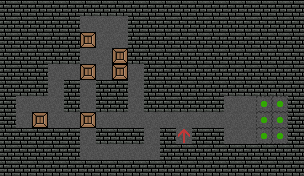
\includegraphics{Original & Extra_1.png}
    \end{frame}

    \section{Résolution}
    \begin{frame}{Test d'arbre}
        \begin{center}
            \begin{tikzpicture}
                [sibling distance=10em,level distance=6em,
                every node/.style={shape=rectangle,draw,align=center}]

                \node{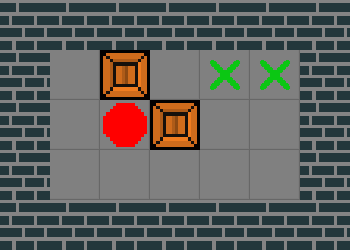
\includegraphics[width=0.2\textwidth]{exhaustive_search/1.png}}
                    child{node{\only<2-3>{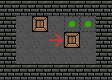
\includegraphics[width=0.2\textwidth]{exhaustive_search/2.png}}}
                        child{node{\only<3>{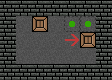
\includegraphics[width=0.2\textwidth]{exhaustive_search/5.png}}}}}
                    child{node{\only<2-3>{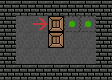
\includegraphics[width=0.2\textwidth]{exhaustive_search/3.png}}}
                        child{node{\only<3>{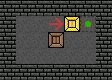
\includegraphics[width=0.2\textwidth]{exhaustive_search/4.png}}}}};
            \end{tikzpicture}
        \end{center}
    \end{frame}
\end{document}
